\documentclass[10pt,letterpaper]{article}

% Preprint layout: full-width title, abstract, and diagram, then a two-column body.
% Not a conference submission and not an arXiv deposit.
\usepackage[T1]{fontenc}
\usepackage{mathptmx}
\usepackage{amsmath}
\usepackage[letterpaper,margin=0.7in,columnsep=0.28in,headheight=14.5pt,headsep=8pt,footskip=24pt]{geometry}
\usepackage{fancyhdr}
\usepackage[font=small,labelfont=bf,labelsep=colon,skip=3pt]{caption}
\usepackage{graphicx}
\usepackage{microtype}

\pagestyle{fancy}
\fancyhf{}
\fancyhead[L]{\footnotesize\itshape MLP, PhysX, and PhysGaussian}
\fancyhead[R]{\footnotesize Preprint}
\fancyfoot[C]{\thepage}
\renewcommand{\headrulewidth}{0.4pt}
\fancypagestyle{plain}{%
  \fancyhf{}%
  \fancyfoot[L]{\footnotesize Preprint}%
  \fancyfoot[C]{\thepage}%
  \renewcommand{\headrulewidth}{0pt}%
}

\makeatletter
\renewcommand{\@seccntformat}[1]{\csname the#1\endcsname.\enspace}
\renewcommand\section{\@startsection{section}{1}{\z@}%
  {-1.7ex \@plus -0.4ex \@minus -0.2ex}%
  {0.7ex \@plus 0.1ex}%
  {\normalsize\bfseries\raggedright}}
\let\savedthebibliography\thebibliography
\renewcommand{\thebibliography}[1]{%
  \savedthebibliography{#1}%
  \footnotesize
  \setlength{\itemsep}{0.15em}%
}
\makeatother

\DeclareRobustCommand{\_}{\textunderscore\allowbreak}
\frenchspacing
\emergencystretch=2em
\sloppy
\newsavebox\titlebox

\begin{document}

\begin{lrbox}{\titlebox}
\begin{minipage}{\textwidth}
\begin{center}
{\Large\bfseries The Physics-Prior MLP with PhysX and PhysGaussian\par}
\vspace{0.4em}
{\large sandy-t-shelvan\par}
\vspace{0.2em}
{10 November 2026\par}
\vspace{0.12em}
{\footnotesize Preprint\par}
\end{center}
\vspace{0.02em}
\begin{center}
{\normalsize\bfseries Abstract}
\end{center}
\begin{quote}
\footnotesize
This note is a design for using the trained per-Gaussian physics prior with NVIDIA PhysX and PhysGaussian~\cite{xie2024physgaussian}.
The joint system has not been run.
The weights in \texttt{data/mlp/physics\_prior\_splat.npz} are epoch 10 of a 14-epoch run in this project.
They correspond to Section 3.4 of Hollis, Fan, and Yang~\cite{hollis2026sceneagent} and are not a released third-party checkpoint.
The MLP runs on each in-mask Gaussian of a fitted splat, and the 33 outputs are averaged.
Rigid, static, and kinematic bodies become PhysX actors.
Soft, cloth, and fluid or granular bodies, and any object whose deformability is at least 0.65, are stepped by PhysGaussian on the same Gaussians.
PhysX contact, from the prior's shape and mass, is the load on those particles.
\end{quote}
\vspace{0.05em}
\begin{center}
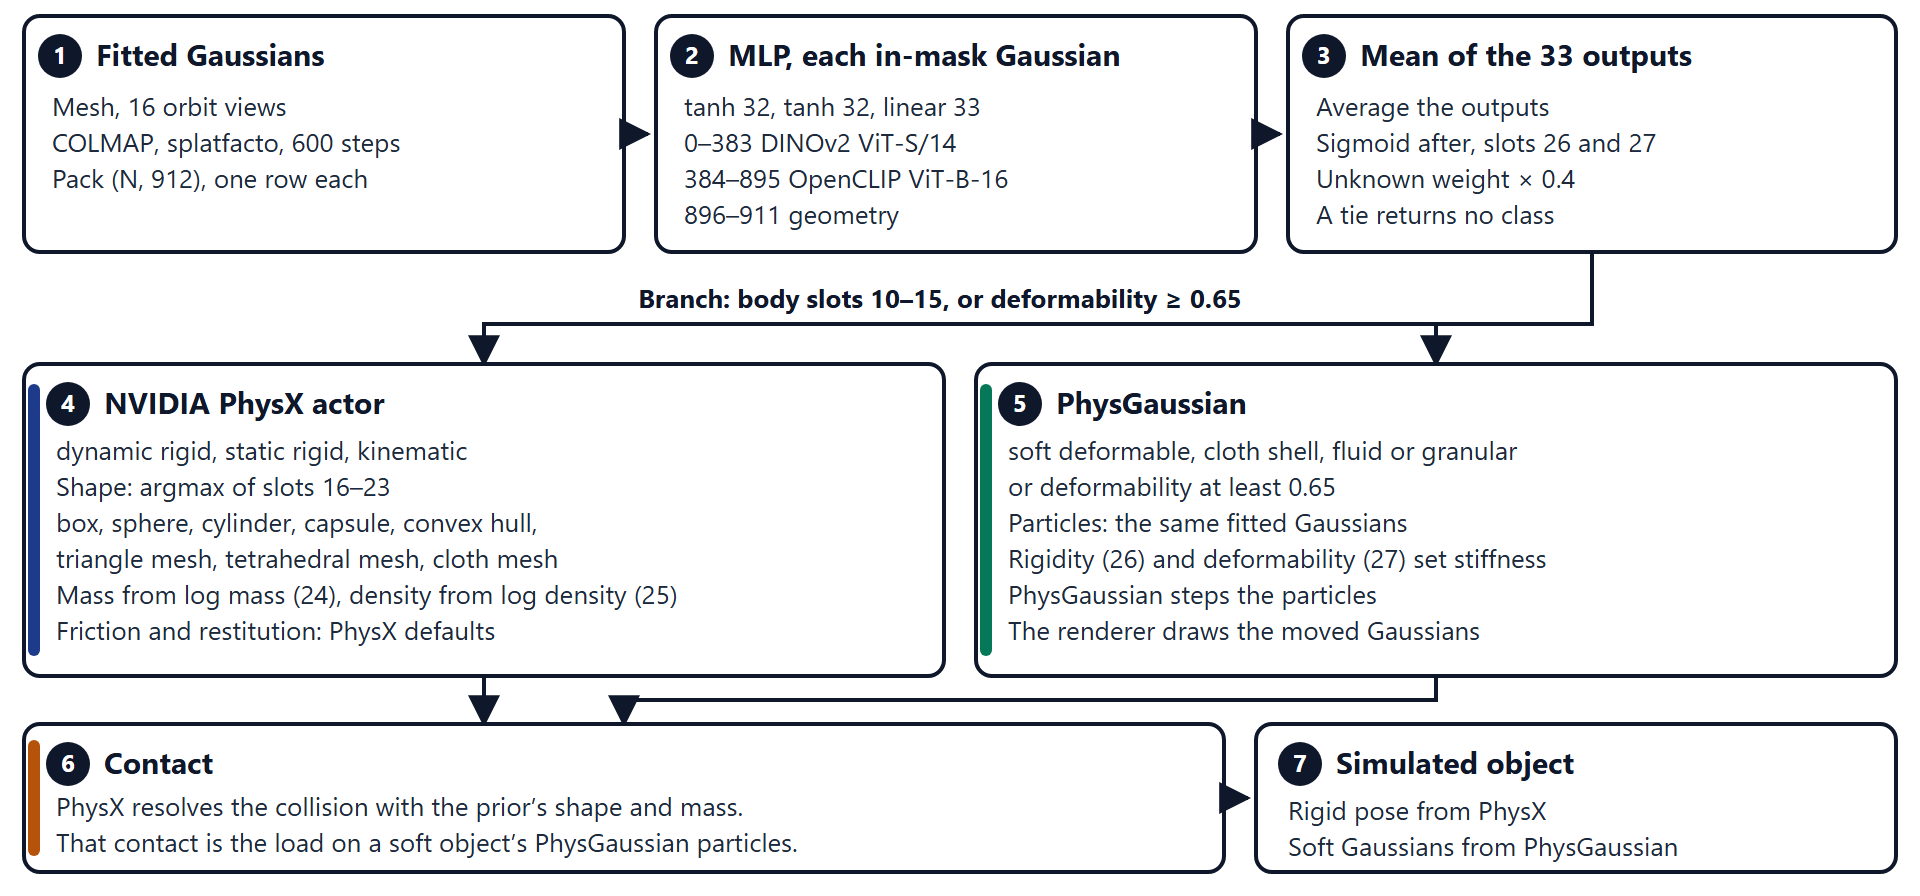
\includegraphics[width=\textwidth]{../docs/figures/mlp_physx_physgaussian.png}\\[0.15em]
{\footnotesize\textbf{Figure 1:} Design of the pipeline. The labels are the trained prior's slots. The joint system has not been run.\par}
\end{center}
\end{minipage}
\end{lrbox}

\twocolumn[\usebox\titlebox]
\thispagestyle{plain}

\section{Fitted splat}
Figure~1 starts from a fitted splat that is already built.
A mesh is rendered as 16 orbit views, eight azimuths at elevations \(18^\circ\) and \(50^\circ\).
COLMAP registers the views, splatfacto fits the Gaussians for 600 steps, and the pack writes \((N, 912)\), one row per Gaussian.
The appearance model is that 3D Gaussian splat~\cite{kerbl2023gaussian}.
A row is kept only when the opacity standard deviation is at least \(10^{-3}\) and the opacity is not the constant 0.99.
The file \texttt{physics\_prior.npz} is not this model.
PhysX later supplies a rigid pose for these kernels.
PhysGaussian writes the moved kernels of a soft object, and the renderer draws them.

\section{Prior}
Columns 0--383 are DINOv2 ViT-S/14.
Columns 384--895 are OpenCLIP ViT-B-16 with the OpenAI weights.
Columns 896--911 are \(x\), \(y\), \(z\), three exp scales, sigmoid opacity, quaternion components \texttt{rot\_0} through \texttt{rot\_3}, DC coefficients \texttt{f\_dc\_0} through \texttt{f\_dc\_2}, log volume, and anisotropy.
The network is \(\tanh\) of width 32, \(\tanh\) of width 32, and a linear head of width 33.
Inference runs that map on every in-mask Gaussian and averages the 33 raw outputs.
Averaging the 912 inputs and running the MLP once is a different function.

The sigmoid is not inside the forward pass.
It is applied to rigidity (slot 26) and deformability (slot 27) after the mean.
A material vote that ties returns no class.
An unknown class weight is multiplied by 0.4.
The keyword proposal is passed in by the caller.
Slots 28--32 stay masked and are unread.
Friction and restitution are null.
Young's modulus, Poisson's ratio, and the rendering material are not predicted.

Slots 0--9 are material logits: plastic, metal, wood, fabric, paper and cardboard, rubber and foam, glass and ceramic, food and organic matter, liquid and granular matter, unknown.
Slots 10--15 are body logits: dynamic rigid, static rigid, kinematic, soft deformable, cloth shell, fluid or granular.
Slots 16--23 are collision logits: box, sphere, cylinder, capsule, convex hull, triangle mesh, tetrahedral mesh, cloth mesh.
Slot 24 is log mass and slot 25 is log density, both natural logs, so the mass in kilograms is \(\exp(y_{24})\) and the density is \(\exp(y_{25})\).
When a physics record is built, sigmoid deformability of at least 0.65 resolves the object as soft deformable.
The body accuracy in Section~\ref{sec:scores} compares the body head with the stored label and does not apply that threshold.

\section{Branch}
The material head does not choose the simulator.
A tie leaves the material class empty and leaves the branch unchanged.
The branch reads the body argmax of slots 10--15, unless sigmoid deformability is at least 0.65.
In that case the physics record names the body soft deformable, and the object takes the PhysGaussian path.
One object yields one 33-dimensional mean, over its in-mask Gaussians.
A scene repeats that mean and the branch once per object.

A body of dynamic rigid, static rigid, or kinematic becomes one NVIDIA PhysX actor.
PhysX is the physics engine that holds that actor.
The collision shape is the argmax of slots 16--23, passed through under that name, including tetrahedral mesh and cloth mesh.
The actor mass is \(\exp(y_{24})\) kilograms and the density is \(\exp(y_{25})\).
Friction and restitution are not predicted, so the actor keeps the PhysX defaults.
Young's modulus and Poisson's ratio are not predicted on this branch.
Dynamic rigid is the actor PhysX integrates under contact.
Static rigid does not move under that contact.
Kinematic keeps a prescribed pose while PhysX still resolves the contact.

A body of soft deformable, cloth shell, or fluid or granular goes to PhysGaussian~\cite{xie2024physgaussian}, as does the deformability rule above.
The particles are the fitted Gaussians.
PhysGaussian's material-point step evolves those same kernels, and the renderer draws the kernels after the step.
Rigidity and deformability, slots 26 and 27, set the stiffness of that step.
The published method also takes continuum constants such as Young's modulus.
This MLP does not predict those constants, so the design passes the two decoded values and does not fill in a modulus or a Poisson's ratio.
The code referred to is \texttt{https://github.com/XPandora/PhysGaussian}.

\section{Contact}
PhysX resolves collisions with the shape from slots 16--23 and the mass from slot 24.
On a dynamic rigid, static rigid, or kinematic actor, that resolution is the actor's contact, and the Gaussians are drawn at the PhysX pose.
On a soft, cloth, or fluid object, the same contact is the external load on that object's PhysGaussian particles.
The collision primitive is the contact shape.
It does not replace the Gaussians, which remain the particles and the drawn kernels.
PhysGaussian then steps the particles, and the renderer draws the moved Gaussians.
A scene may contain both kinds of object.
Each step resolves the PhysX contact, applies that load on the soft branch, steps those particles, and draws the simulated object: the PhysX pose of each rigid actor together with the Gaussians PhysGaussian has moved.
This coupling is a design.
It is not implemented in this repository, and it has not been run.

\section{Scores of the MLP alone}
\label{sec:scores}
The only measured numbers here are attribute scores of the restored epoch-10 MLP.
The test split has \(n = 323\).
It was scored once, after validation had already chosen epoch 10, and it did not choose the epoch.
The test loss is 2.088, material accuracy is 0.889, body accuracy is 0.991, and collision accuracy is 0.768.
Those three accuracies are fractions of test objects whose argmax matches the stored label.
They are attribute scores of the prior.
They are not a PhysX metric and they are not a PhysGaussian metric.
The joint system has not been scored.
The full values are in \texttt{data/mlp/train\_report\_splat.json}.

\begin{thebibliography}{9}

\bibitem{kerbl2023gaussian}
Bernhard Kerbl, Georgios Kopanas, Thomas Leimk{\"u}hler, and George Drettakis.
3D Gaussian Splatting for Real-Time Radiance Field Rendering.
\textit{ACM Transactions on Graphics}, 42(4), 2023.

\bibitem{hollis2026sceneagent}
Hollis, Fan, and Yang.
SceneAgent: An Agentic Pipeline from 3D and 4D Captures to Simulation Environments.
Harvard Computational Robotics Group, preprint, 2026.
arXiv:2610.34745.

\bibitem{xie2024physgaussian}
Tianyi Xie, Zeshun Zong, Yuxing Qiu, Xuan Li, Yutao Feng, Yin Yang, and Chenfanfu Jiang.
PhysGaussian: Physics-Integrated 3D Gaussians for Generative Dynamics.
In \textit{Proceedings of the IEEE/CVF Conference on Computer Vision and Pattern Recognition (CVPR)}, pages 4389--4398, 2024.

\end{thebibliography}

\end{document}